\chapter{Influence of loss of control}
\label{chap:loc}

\lettrine{I}{t} is widely believed that \ac{BCI} performance fluctuates over
time due to non-stationary feature distributions \cite{mueller2008mlr,
blankertz2007ics, bunau2009ssa, vidal1977rtd, shenoy2006tac, krauledat2008tzt,
sun2006afe, wolpaw2002bci, jatzev2008ecn}. These non-stationary feature
distributions violate the basic assumption made by the classification models
that the evaluation data (i.e. the online session) is distributed identically
to the data the model was trained on. This problem is known as \emph{covariate shift}, and leads to decreases in the classification performance.
%
Among the hypothesised causes for these non-stationary feature distributions
are changes in the mental state (e.g. fatigue, workload, \ac{LOC}) and
artifacts \cite{blankertz2007ics, jatzev2008ecn}.
\todo{DH: Is LOC een bestaand concept -> kun je meer over zeggen}
%
Although it seems plausible that mental state changes that are detectable in
the \ac{EEG} can interfere with \ac{BCI} operation, there is not much
experimental evidence for this effect. 

In this Chapter, we therefore describe an experiment\footnote{ The work
described in chapter was accepted for publication in the journal IEEE
Transactions of Neural Systems and Rehabilitation Engineering
\cite{reuderink2011ilc}.} we performed to investigate the influence of a
feeling of \ac{LOC} on the detectability of movements with the left and right
index finger through the \ac{EEG}. 
%
Changes in the \ac{EEG} related to users experiencing a state of \ac{LOC} might
lead to a decrease in \ac{BCI} performance due to the aforementioned covariate
shift. In turn, the user state is again influenced by the decreased performance
of the \ac{BCI}; for example, the non-working \ac{BCI} could cause increased
frustration, anger and reduced alertness. This interaction between the user
state and the \ac{BCI} performance might result in a positive feedback loop,
leading to a \ac{BCI} that spins out of control.
%
Given the huge drawbacks of a \ac{BCI} that can stop working depending on the
mental state of a user, understanding the influence of changes in the mental
state on the \ac{BCI} is of great importance to develop reliable \acp{BCI}.

In the following sections we will describe previous work on the relation between
mental states and \ac{BCI} performance, the methods we used, our results, and a
discussion of our experiment, followed by conclusions and directions for future
research.

\section{Previous work}
The influence of frustration associated with \ac{LOC} on a
\ac{BCI} is of great interest since it might cause the previously described
feedback loop. This influence  was previously investigated in
\cite{jatzev2008ecn, zander2009usi}. In this study, users were instructed to
use real movement with their left or right hand to rotate respectively L or
R-shaped objects to a target position in order to study the effect of \acl{LOC}
on the \ac{BCI} performance.
%
The color of the letter indicated the angle of rotation, and the user could
press a key to rotate the object in the direction indicated by the shape of the
object every second.
%
After performing a calibration block with cued left/right hand movement and two
practise blocks with this so-called RLR paradigm, a \ac{LOC} was simulated in
the third block by occasionally using a wrong angle of rotation in the
application. Both an \ac{ERD} and an \ac{ERP} based classifier were trained on
the first block, and applied to the other blocks in an off-line analysis.  A
significant difference between the training block and the \ac{LOC} block was
found for the distribution of \ac{ERD} based features, but for \ac{ERP}
features no such difference was found. This seems to indicate that there is
variability in \ac{ERD} features related to \acl{LOC}. 

However, the study described in \cite{jatzev2008ecn, zander2009usi} is lacking
on a few aspects. Most notable is the limitation that changes in \ac{BCI}
performance due to the induction of \ac{LOC}, the progression of time,
differences in stimulation and user behaviour cannot be distinguished.
%
We were interested in the influence of \ac{LOC} on the \ac{BCI} performance
independent of these other factors. Therefore we used 1) an interleaved block
design to control for effects that manifest spontaneously over time, such as
increasing fatigue, changing temperature, drying gel on the electrodes etc., 2)
we used the same environment for training and evaluating the \ac{BCI}
classifiers to minimize environmental differences not related to \ac{LOC}, 3)
we used self-reported emotional ratings to validate the effect of \acl{LOC} on
the mental state and 4) we tested and corrected for confounding behavioural
changes, such as changes in the force, speed or order of the finger movements,
and eye movements. 

\section{Methodology}
To study the effect of \acf{LOC}, we designed a Pacman game that periodically
reduced the amount of control the user has over his avatar.
The \ac{EEG} was passively recorded during game play, and afterwards the
off-line performance of an \ac{ERD} and an \ac{ERP} based classifier was used to
assess the influence of \ac{LOC} on the \ac{BCI} performance. In the rest of
this section, we describe the data collection, the preprocessing and
classification of the \ac{EEG}, and the evaluation method in more detail.

\subsection{Data collection}
%\subsubsection{The Pacman Game}\label{sec:affpac}
A game was designed to induce a state of \ac{LOC}, with game play similar to
the original Pacman game \cite{reuderink2009apf}. The major differences with
other Pacman games is that our game periodically tried to induce a state of
\ac{LOC} in the user by responding unreliably to the keyboard commands. Since
unreliable input is a proven method for frustration induction
\cite{scheirer2002fup, klein2002cru, diener2006eaa}, we expected this method to
induce mental state changes that were naturally associated with \ac{LOC}.
%
To simplify (simulated) \ac{BCI} control, the user input was reduced to a
button for the left index finger that turned Pacman 90 degrees counterclockwise,
and a button for the right index finger that turned Pacman clockwise. 

\begin{figure}
  \centering
  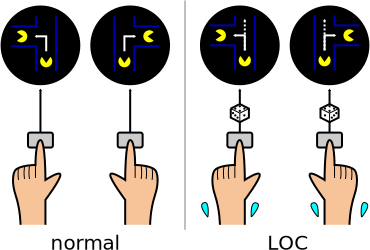
\includegraphics[width=2in]{experiment_figure}
  \caption{In the normal condition, the left button rotated the player
  $90^{\circ}$ counterclockwise; the right button rotated the player
  $90^{\circ}$ clockwise. In the \protect\ac{LOC} condition, 15\% of the
  keyboard input was ignored, and a visual lag was induced (not shown).}
  \label{fig:experiment_concept} 
\end{figure}

\subsubsection{Experiment design}
The \ac{LOC} was induced in a randomized interleaved block design with
experimental blocks of two minutes. In one third of these two-minute blocks
\ac{LOC} was induced, in the other blocks the game play remained unmodified.
The \ac{LOC} blocks were evenly distributed over the session by building a
series of shuffled sequences of three blocks (one \ac{LOC} and two normal
blocks). In the \ac{LOC} condition, the game randomly ignored 15\% of the keystrokes, resulting in a barely playable game. In addition, the display
occasionally lagged in the \ac{LOC} condition. After each block, the user was
asked to rate his mental state in terms of valence (pleasure), arousal and
dominance (subjective feelings of control) on a Likert-scale presented under
the \ac{SAM} \cite{bradly1994mes}.

\subsubsection{Experimental procedure}
Subjects were asked to read and sign a form of consent, and were subsequently
wired with the \ac{EEG} and physiological sensors. The experimenter briefly
explained the game and the self-assessment procedure. The subject was
allowed to practise the controls for two minutes before the experiment was
started. If users mentioned that the game was unresponsive during the
experiment, the experimenter asked them to continue playing and promised to
find the cause later. After 30 minutes, the experimenter stopped the experiment
and the users were debriefed.

\subsubsection{Sensors and recording}
\begin{sloppypar}
A BioSemi ActiveTwo \ac{EEG} system was used to record the \ac{EEG} and
physiological signals at a sample rate of 512~Hz. \Ac{EEG} was recorded with 32
Ag/AgCl active electrodes placed at locations of the Extended International
10-20 system. To measure the influence of ocular and muscle artifacts, we
recorded the \acs{EOG} (horizontal and vertical pairs) and two pairs of
\acs{EMG} signals over the left and right flexor digitorum profundus (the
muscles used to press with the index finger).  Additional physiological
sensors, such as temperature, respiration, the galvanic skin response and the
blood volume pulse were recorded as well, but not used in the present
study\footnote{The recordings are available at
\url{http://borisreuderink.nl/perm/affpac/}.}.
\end{sloppypar}

\subsection{Preprocessing}
The following preprocessing procedure was applied to reduce the influence of
noise and artifacts caused by eye movements and muscle tension: first the
recording was downsampled to 128 Hz to speed up processing. After downsampling,
the data was high-pass filtered using a 4th-order Butterworth filter to remove
frequencies below 0.2 Hz, and notch-filtered using a 4th-order Butterworth
filter from 49--51 Hz to remove power line noise. The \ac{EEG} was then
corrected for eye movements using a regression  based subtraction
method \cite{schloegl2007fac}.
To prevent noise from spreading to other channels, we performed
channel-level preprocessing before we applied the \ac{EOG} correction and
re-referenced the signals to the \ac{CAR}.

\subsection{Key press classification from EEG}
\begin{sloppypar}
Most motor imagery based \acp{BCI} are based on sensory-motor rhythms,
specifically the \acf{ERD} that occurs during both real and imaginary movement.
As the \ac{ERD} of real and imagined hand movement is similar
\cite{mcfarland2000mbr}, we used real movement to train \acp{BCI} that predict
the movement from the \ac{EEG} signal, since it provides a clear ground truth
and allows for a tighter controlled experiment. In this section we will outline
the classifiers used for detection of the \ac{ERD} and the \ac{ERP} associated
with the movements executed to play the game.
\end{sloppypar}

\subsubsection{\protect\ac{ERD} features}
\begin{sloppypar}
The \ac{ERD} classification was based on the decrease in the Rolandic mu rhythm
(8--12~Hz) and Rolandic beta frequencies (peak around 20~Hz) on the
contra-lateral motor cortices that occurs when movement is initiated
\cite{pfurtscheller1999eem}.
% 
After preprocessing, we applied a 6th-order Butterworth band-pass filter to
extract the frequencies from 8--30 Hz, which includes both the mu and beta
rhythms. From this filtered \ac{EEG} we extracted windows of one second,
centered on the moment that keystroke was registered. Visual inspection
confirmed that an \ac{ERD} did indeed occur within this period. For these
segments we trained subject-specific spatial filters with the \ac{CSP}
algorithm.
\end{sloppypar}

The \ac{CSP} algorithm \cite{koles1991qet} finds a matrix $\tilde{W}$ with
spatial filters that map the \ac{EEG} into a new space with basis vectors that
have a high variance for the first class and a low variance for the second, and
vice versa. Given the number of sensors $s$, and the number of samples $n$,
$W$ is an $s \times s$ transformation matrix with the following property:
%
\begin{equation}
  \Sigma_{WX_1} = D \quad \textrm{and} \quad
  \Sigma_{WX_1} + \Sigma_{WX_2} = I, 
  \label{eq:CSP_BR}
\end{equation}
%
where $D$ is a diagonal matrix with elements in descending order, $I$ is
the identity matrix and $\Sigma_{X_i}$ is the channel covariance matrix of the
$s \times n$ \ac{EEG} measurements matrix $X$ for given class $i$.
%
Rows of $W$ that correspond to a high value in $D$ have a high variance (power)
for the first class and a low variance for the second, and vice versa. Because
of this discriminatory property, the $\frac{m}{2}$ first and the $\frac{m}{2}$
last rows were picked to construct the final matrix $\tilde{W}$ with $m=6$
spatial filters.

After applying the \ac{CSP} algorithm, we calculated the variance (which
corresponded to the band power in the mu and beta band) for each transformed
channel, which resulted in $m$ spatial band-power features.

\subsubsection{\protect\acs{ERP} features}
A less frequently used paradigm for classification of \ac{EEG} related to
movement is based on the \ac{BP}, a negative \ac{ERP} related to movement
initiation. The \ac{BP} consists of an early phase beginning about 2 seconds
before the movement onset, and a late phase with a steeper slope 400~ms before
the onset \cite{shibasaki2006wb}.  We used the asymmetric distribution of the
late \ac{BP} over the scalp for classification of the laterality of the hand
movements, which is known as the \ac{LRP}.

For the \ac{ERP} classification, we used the same preprocessing pipeline as
used with the \ac{CSP} classification up to the band-pass filter. Then we
applied a (4th-order Butterworth) low-pass filter at 10~Hz, and again extracted
windows of one second centered on the moment of registration of keyboard
input. These trials were then transformed with a whitening transform $P$
which has the property that the transformed signals are uncorrelated, and have
unit variance:
%
\begin{equation} 
  \Sigma_{PX} \approx P \Sigma_X P^T = I.  
\end{equation}
%
With the eigenvalue decomposition $\Sigma_X = U \Lambda U^T$, we find that
%
\begin{equation}
  P = \Lambda^{-\frac{1}{2}} U^T. 
\end{equation}

After whitening with $P$, we downsampled the signal by taking every fourth
sample point, resulting in a $s \times \frac{e}{4}$ feature vector where
$e=128$ is the number of samples in a classification window.
%
Despite superficial differences, this method for \ac{LRP} classification is
conceptually similar to the conventional approaches for \ac{ERP} detection,
such as \cite{blankertz2003bbr, blankertz2011sta}, but does not rely on time
segment or channel picking.

\subsubsection{Classification}
The \ac{ERD} and \ac{LRP} features were used to train a final linear \ac{SVM}
classifier. The \ac{SVM}'s regularization parameter $c$ was selected with a
separate cross-validation loop on the two-minute blocks in training set. 

\subsection{Loss of control analysis} \label{sec:dga}
\begin{sloppypar}
To analyze the influence of user \ac{LOC} on the performance of a \ac{BCI},
we trained a \ac{BCI} on normal blocks, and measured the difference in
performance of the same classifier between unseen, normal blocks and unseen
blocks from the \ac{LOC} condition.
% 
As we could not assume that the distribution of the \ac{EEG} signal
would remain stationary, training and evaluating a \ac{BCI} on samples uniformly
spread over the sessions might lead to an overestimation of the performance.
In order to have a more reliable measure of how an online \ac{BCI} would
perform, we therefore used a special evaluation scheme where complete
experimental blocks were left out for evaluation:
%
The session consisted of a series of permutations of three experimental blocks;
two normal blocks, and a block with \ac{LOC} simulation. For every three
blocks, we added the first normal block to the training set for the \ac{BCI}
classifier. The remaining normal and \ac{LOC} block were used for evaluation.
This way, the training data was spread over time, but we still have independent
blocks for evaluation.
%
Note that this evaluation is not symmetrical, since the classifiers were
trained only on normal blocks, but tested on blocks of both the normal and
\ac{LOC} condition. 
\end{sloppypar}

If there were difference between the normal and \ac{LOC} conditions, we
expected to find a lower performance on \ac{LOC} blocks compared to block with
normal control, since the model was optimized for a different distribution than
the observations it was evaluated on had.

\subsection{Performance measure}
\ac{BCI} classifiers are often evaluated by comparing their accuracy on
out-of-sample trials. The choice for the accuracy measure is problematic, as
accuracies (or equivalently, error rates) are hard to interpret when the prior
probabilities of the classes are unequal and/or variable. Furthermore, the
statistic does not take the time needed to perform a trial (key press) into
account: due to our short \acp{ITI}, lower accuracies were to be expected for
our \acp{BCI} than the accuracies reported for more traditional \ac{BCI}
environments, where multiple seconds are used to detect an imagined movement.
Despite these drawbacks, we will provide accuracy measures because it is
commonly used.

\begin{sloppypar}
A more informative measure is the \ac{ITR}, which conveniently captures the
amount of information a user can communicate through a (noisy) channel with an
optimal encoding strategy. It does so by combining the quality of and the time
needed for the predictions. As such, the \ac{ITR} is a better measure to
evaluate \ac{BCI} performance.
%
Note that different formulas to calculate the \ac{ITR} are used in the \ac{BCI}
literature, for example Wolpaw's definition in \cite{wolpaw2002bci} is often
used. The drawback of this definition is that it has a number of assumptions
that are often violated in practice, most notably the assumption that all
classes have the same prior probability. The \ac{ITR} based on \ac{MI} does not
rely on these assumptions, hence we use \ac{MI} to measure the information
contained in the prediction of a single trial. Note that the labels of the
trials still need to be independent of each other for a correct estimate of the
\ac{ITR}.
\end{sloppypar}

The \Ac{MI} expresses the decrease in uncertainty of a discrete variable
$\mathcal{Y}$ (the true labels), given a discrete variable $\mathcal{Z}$ (the
predictions of the classifier):
%
\begin{equation} \label{eq:mi} I(\mathcal{Z}; \mathcal{Y}) = \sum_{\substack{y
\in \mathcal{Y}\\z \in \mathcal{Z}}} p(z, y) \log_2{\frac{p(z,
y)}{p_1(z)\,p_2(y)}}, \end{equation}
%
where $p(z, y)$ is the joint probability distribution and $p_1(z)$ and $p_2(y)$
are the marginal probability distribution functions of $\mathcal{Z}$ and
$\mathcal{Y}$. With the base-2 logarithm the reduction in uncertainty is
expressed in bits. We use the \ac{MI} between the classifiers predictions and
the ground truth as a second performance measure. The joint and marginal
probabilities in \eqref{eq:mi} were estimated by their relative frequency of
occurrence in the confusion matrix.

Finally, we calculate the third measure \ac{ITR} $R$, in bits per minute, based on the
\ac{MI} \eqref{eq:mi}, and the median\footnote{We use the median instead
of the mean because $\Delta t$ appeared to follow a Poisson distribution.} \acl{ITI} $\med(\Delta t)$:
%
\begin{equation}
  R = 60 \frac{I}{\med(\Delta t)}.
\end{equation}

As a fourth, and last performance measure, we use the \ac{AUC} of the \ac{ROC}
\cite{fawcett2005ira} to express the ranking performance of the classifier. The
\ac{AUC} is equal to the probability that a randomly chosen instance of the
first class is ranked above a randomly chosen instance of the second class;
in other words, an \ac{AUC} of 0.5 indicates random performance, and an
\ac{AUC} of 0 or 1 indicates perfect ranking ability. Like the \ac{MI}, the
\ac{AUC} does not assume equal prior probabilities.

Originally we planned to use the \ac{KLD} as a measure of change in the feature
distributions as in \cite{shenoy2006tac}, but the assumption that the features
are normally distributed was violated heavily by both our \ac{ERD} features
(even after log-transforming) and our \ac{LRP} features. This made the
estimation of the \ac{KLD} unfeasible due to the need for high-dimensional
density estimation.


\subsection{Confounding factors}
\begin{sloppypar}
To induce mental state change associated with \ac{LOC}, we intentionally
degraded the quality of control. Behavioural changes (e.g. repetitive and
force-full keystrokes, and more frequent gazing at the hands) might have
occurred as a result of the method of induction. Therefore, potential
differences in \ac{BCI} performance might have been caused solely by these
changes in behaviour. In this context, behavioural changes are confounding
factors, and need to be corrected for. 
\end{sloppypar}

However, we cannot discern behavior caused by the method of induction and
behaviour caused by induced changes in the mental state. Correcting for
confounding factors could therefore reduce the variation in mental state, and
lead to an underestimation of the effect. Therefore, we performed our analysis
both with and without correction for confounding behaviour.

\begin{sloppypar}
Behavioural changes that we identified as confounding factors were the \acf{ITI},
the repetition of keystrokes with the same hand, the fraction of keystrokes
per hand, the force used to press a key, and eye
movements.
%
The \ac{ITI} can be confounding because the \ac{EEG} is analyzed over a short
period of time; keystrokes that follow each other quickly could lead to
masking of relevant \ac{EEG} features, or worse, to the leaking of label
information from one keystroke to the next.
Repetition of strokes with the same hand might lead to increased performance
for the same reason.
%
Force is a confounding factor because force has an influence on the \ac{ERD}
\cite{stancak1997eel}.
%
Artifacts related to eye movements are known to have a profound influence
on \ac{EEG} analyses, but these were (greatly) attenuated by the \ac{EOG}
regression method during preprocessing.
\end{sloppypar}

% how do we correct?
To correct for the confounding factors, we used multi-variate frequency
matching. Frequency matching involves stratifying the distribution of the
confounding variable, and drawing samples such that the number of samples
within each stratum is the same per condition \cite{anderson1980smc}. In our
case, the multivariate distributions of the previously described confounding
variables in the normal and \ac{LOC} conditions were matched.

% measuring the confounds
These confounding factors were quantified as follows. To quantify the \ac{ITI},
we used the logarithm of the difference in seconds between consecutive trials.
The keystroke patterns were modeled with a discrete bivariate distribution of
the label of the current and previous trial. For force, a bivariate (i.e. left
and right arm's \acs{EMG} power) distribution of the log-transformed \ac{EMG}
power was used. To calculate the \ac{EMG} power, the procedure outlined in
\cite{hof1984emg} was used: 
%
1) apply a high-pass filter with a cut-off of 30~Hz, 2) apply the Hilbert
transform to extract the envelope of the signal and 3) apply a low-pass filter
with a cut-off of 40~Hz to smooth the signal. 

A multi-dimensional histogram with regularly spaced bins was used to extract
strata for frequency matching: 4 bins were used for log \ac{ITI}, $2 \times 2$
bins were used for label patterns, and $5 \times 5$ bins were used for log
\ac{EMG} power for index fingers.

\subsection{Statistical tests}
\begin{sloppypar}
Comparisons over subjects were performed using Wilcoxon signed-rank tests, on
pairs of per-condition averages for each subject. This test is a
non-pa\-ra\-me\-tric alternative to the commonly used paired Student's t-test,
which could not be applied because the t-test's assumptions that the
measurements are normally distributed and have equal variances do not hold for
classification performance \cite{demsar2006scc}. 
\end{sloppypar}

In addition to this over-subjects analysis, we performed a more sensitive meta
analysis that combines the within-subject $p$-values to test for individual
differences (as opposed to group differences). It combines the  $p$-values of
different subjects to reject the combined null hypothesis $H_0$, that states
that each of the individual null hypotheses is true. The combined alternative,
$H_A$, is that at least one is not true. For this purpose, Fisher's method was
suggested in \cite{loughin2004scm} for combining $p$-values:
%
\begin{equation} X^2 = -2 \sum_{i=1}^{k}\log_e{p_i}, \end{equation}
%
where $p_i$ is the $p$-value for subject $i$. When the null hypotheses are all
true, and the $p_i$'s are independent, $X^2$ follows a $\chi^2$ distribution
with $2k$ degrees of freedom. Note that opposing effects might be combined in a
significant outcome with the Fisher's method if two-sided tests are used.

We used a significance level $\alpha = 0.05$ for all tests presented in this
chapter. 

\section{Results}
\subsection{Subjects}
Twelve healthy users (age $27 \pm 3.9$) participated in the experiment.  All
participants had normal, or corrected to normal vision, and reported not to use
medication. Only three of our subjects were female, and all subjects were
right-handed. Most participants had some video game experience, and four
subjects had previous experience with \acp{BCI}.

\subsection{Self assessments}
To verify the induction of changes in the mental state, we analysed the self
reported emotional ratings of the \ac{SAM}. Most subjects rated the \ac{LOC}
condition more negatively than the normal condition, over subjects this
difference was significant ($T$=3, $p$\textless 0.01). While we expected to
find a trend towards more arousal in the \ac{LOC} condition, there was no
significant difference ($T$=23, $p$=0.26). The dominance dimension, which
measures the amount of dominance, or control they have on their environment,
indicate that people seemed to be significantly ($T$=3.5, $p$\textless 0.01)
more in control in the normal condition.


\begin{figure}
  \center
  \includegraphics[width=3.5in]{key_duration.pdf}
  \caption{The histogram for the time between key presses during game play for
  all subjects. The intervals for the normal condition are displayed in black,
  the \protect\ac{LOC} condition is displayed in red (gray). The histogram is
  dominated by short $\Delta t$'s between key presses. The histogram of the
  \protect\ac{LOC} condition seems to be slightly more pinched around half a
  second.}
  \label{fig:key_duration}
\end{figure}

\begin{figure}
  \center
  \includegraphics[width=3.5in]{emg_cond.pdf}
  \caption{The mean log \protect\ac{EMG} power and its standard deviation
  (dashed lines) is displayed for both the normal and \protect\ac{LOC}
  condition, time-locked to the key press at $t=0$. The top plot shows the EMG
  power of the left bipolar channel for left index-finger presses, the bottom
  plot show the EMG power for right hand movement measured with the right
  bipolar channel.}
  \label{fig:emg_cond}
\end{figure}

\begin{table}
  \caption{Statistics of confounding variables. The repetitiveness (second
  column) and log-\protect\ac{EMG} power (last column) differ significantly
  between the conditions. The \protect\ac{EMG} power was quantified as the
  maximum power in the interval [-0.2,~0]~s. The start and end of the arrow
  signify the mean value in the normal and \protect{LOC} condition
  respectively.} 
  \center \footnotesize
  \begin{tabular}{c c c c c}
\toprule
 & log $\Delta t$ & $p(y_t=y_{t-1})$ & log pow. EMG L & log pow. EMG R\\
\midrule
S0 & -0.48 $\rightarrow$ -0.36 &  0.51 $\rightarrow$  0.59 &  1.31 $\rightarrow$  1.21 &  1.08 $\rightarrow$  1.15\\
S1 & -0.51 $\rightarrow$ -0.53 &  0.54 $\rightarrow$  0.59 &  2.70 $\rightarrow$  2.60 &  2.04 $\rightarrow$  2.17\\
S2 & -0.54 $\rightarrow$ -0.59 &  0.50 $\rightarrow$  0.52 &  2.65 $\rightarrow$  2.58 &  2.51 $\rightarrow$  2.46\\
S3 & -0.47 $\rightarrow$ -0.61 &  0.56 $\rightarrow$  0.54 &  1.99 $\rightarrow$  1.88 &  2.15 $\rightarrow$  2.31\\
S4 & -0.46 $\rightarrow$ -0.55 &  0.53 $\rightarrow$  0.58 &  3.14 $\rightarrow$  3.35 &  1.76 $\rightarrow$  1.86\\
S5 & -0.46 $\rightarrow$ -0.44 &  0.56 $\rightarrow$  0.60 &  2.70 $\rightarrow$  2.56 &  4.06 $\rightarrow$  3.91\\
S6 & -0.46 $\rightarrow$ -0.48 &  0.55 $\rightarrow$  0.55 &  2.11 $\rightarrow$  2.55 &  2.14 $\rightarrow$  2.47\\
S7 & -0.40 $\rightarrow$ -0.55 &  0.58 $\rightarrow$  0.56 &  1.70 $\rightarrow$  1.71 &  2.13 $\rightarrow$  2.14\\
S8 & -0.37 $\rightarrow$ -0.44 &  0.47 $\rightarrow$  0.56 &  2.89 $\rightarrow$  2.95 &  2.94 $\rightarrow$  3.02\\
S9 & -0.58 $\rightarrow$ -0.55 &  0.45 $\rightarrow$  0.54 &  3.02 $\rightarrow$  3.08 &  2.01 $\rightarrow$  2.06\\
S10 & -0.58 $\rightarrow$ -0.44 &  0.47 $\rightarrow$  0.53 &  2.43 $\rightarrow$  2.42 &  2.52 $\rightarrow$  2.55\\
S11 & -0.45 $\rightarrow$ -0.42 &  0.52 $\rightarrow$  0.58 &  3.01 $\rightarrow$  2.86 &  2.97 $\rightarrow$  3.13\\
\midrule
mean & -0.48 $\rightarrow$ -0.50 &  0.52 $\rightarrow$  0.56 &  2.47 $\rightarrow$  2.48 &  2.36 $\rightarrow$  2.44\\
Wilc. & T=32, p=0.583 & \textbf{T=6, p=0.010} & T=31, p=0.530 & \textbf{T=12, p=0.034}\\
\bottomrule
\end{tabular}

  \label{tab:confounds} 
\end{table}

\subsection{Confounding behavioural differences} \label{sec:behav} 
In this section we describe the analysis of the characteristics of the user's
behaviour, as it might have had a confounding influence on the \ac{BCI}
performance. 
%
Both differences in the \ac{ITI}, and the pattern of consecutive keystrokes
can indicate a confounding behavioural change. The per-subject statistics for
these confounding factors are presented in Table~\ref{tab:confounds}. For the
log \ac{ITI}, we see an insignificant tendency to shorter intervals between key
presses in the \ac{LOC} condition. The probability that a key press was made
with the same hand is significantly higher in the \ac{LOC} condition. This may have been caused by increased repetition, by increased imbalance of the class ratios,
or a combination thereof. Nevertheless, it indicates a significant behavioural
change.

The temporal development of the \ac{EMG} signal is displayed in
Fig.~\ref{fig:emg_cond}. An increase in the \ac{EMG} power is visible just
before the stroke is registered, and a much weaker increase is visible when the
key is released. Most of the activity is registered in the interval [-0.2, 0]~s
relative to the registration of the key press. We used the maximum \ac{EMG}
power in this interval to estimate the force used to press a key (see
Table~\ref{tab:confounds}). Movements with the right index finger produce
significantly more \ac{EMG} power in the \ac{LOC} condition.

\begin{figure}
  \center
  \includegraphics[width=\textwidth]{eog_cond.pdf}
  \caption{The vertical eye movement (first row) show downward eye-gaze just
  after a keystroke at $t=0$. The horizontal bipolar \protect\ac{EOG} channel
  is rather uneventful, only for right hand movement (last column) does there
  appear to be a delayed reaction to the key press, first negative (looking
  left) then positive (looking right). The dashed lines indicate the standard
  deviation.  There is no significant difference (16 point Bonferroni corrected
  Wilcoxon signed-rank test over subjects) between the normal (black) and
  \protect\ac{LOC} condition (red).}
  \label{fig:eog_cond}
\end{figure}

Although we removed (most) of the influence of the \ac{EOG} signal from the
\ac{EEG}, it is interesting to look at the user's gaze and blink behaviour
during a key press (Fig.~\ref{fig:eog_cond}). We can see that users tend to
look at their hands 200~ms after a key press, which is most visible in the
vertical \ac{EOG}, and at 300~ms, the variability of the vertical \ac{EOG}
signal seems to increase. This might be caused by eye-blinks, or an adjustment
to the new movement direction of the avatar in the game. 

In summary, our behaviour analysis has shown that the normal and
\ac{LOC}-con\-di\-tions are very similar in the timing, the predictability of
the key\-strokes, the amount of force used to press the keys, and in eye
movements. However, there was a small but significant increase in repetition of
the same movement, and a small significant increase in the force used with the
right hand. After balancing the confounding variables and their interactions
per subject, on average 25\% of the original trials were removed.

\subsection{Impact of loss of control on the BCI}
To investigate the influence of \ac{LOC} on the \ac{BCI} performance, we
trained the \ac{ERD} based and the \ac{ERP}-based classifier on blocks from the
normal condition, and compared the performance on unseen normal blocks with the
performance on blocks from the \ac{LOC} condition. Please refer to
Section~\ref{sec:dga} for more information on this procedure.

\begin{table*} 
  \caption{The influence of \protect\ac{LOC} on a \protect\ac{CSP} classifier
  is shown below, without correction for confounding factors. The start and end
  of the arrow indicate the median performance for the normal and
  \protect\ac{LOC} condition respectively. The $p$-value of a Mann-Whitney U
  test on the per-block performance is displayed above the arrow. The row
  denoted with ``Wilc.'' signifies the over-subject comparison with the Wilcoxon
  signed rank test. The row denoted by ``Fish.'' presents the results of
  combining one-sided $p$-values for an increase in performance.}
  \center \scriptsize
  \begin{tabular}{c c c c c}
\toprule
 & Accuracy & AUC & MI & ITR\\
\midrule
S0 &  0.679 $\xrightarrow{p=0.35}$  0.736 &  0.759 $\xrightarrow{p=0.35}$  0.843 &  0.110 $\xrightarrow{p=0.35}$  0.193 & 11.680 $\xrightarrow{p=0.48}$ 13.763\\
S1 &  0.599 $\xrightarrow{p=0.48}$  0.618 &  0.616 $\xrightarrow{p=0.64}$  0.652 &  0.021 $\xrightarrow{p=0.64}$  0.041 &  2.601 $\xrightarrow{p=0.64}$  4.525\\
S2 &  0.619 $\xrightarrow{p=0.92}$  0.555 &  0.543 $\xrightarrow{p=0.62}$  0.578 &  0.001 $\xrightarrow{p=0.77}$  0.000 &  0.088 $\xrightarrow{p=0.92}$  0.025\\
S3 &  0.474 $\xrightarrow{p=0.13}$  0.519 & \textbf{ 0.466 $\xrightarrow{p=0.05}$  0.518} &  0.004 $\xrightarrow{p=0.62}$  0.003 &  0.452 $\xrightarrow{p=0.77}$  0.338\\
S4 &  0.519 $\xrightarrow{p=0.92}$  0.507 &  0.549 $\xrightarrow{p=0.92}$  0.526 &  0.002 $\xrightarrow{p=0.77}$  0.003 &  0.224 $\xrightarrow{p=0.77}$  0.351\\
S5 &  0.741 $\xrightarrow{p=0.92}$  0.750 &  0.828 $\xrightarrow{p=0.92}$  0.832 &  0.167 $\xrightarrow{p=0.92}$  0.188 & 15.616 $\xrightarrow{p=0.92}$ 20.297\\
S6 &  0.538 $\xrightarrow{p=0.65}$  0.529 &  0.543 $\xrightarrow{p=0.86}$  0.522 &  0.003 $\xrightarrow{p=0.59}$  0.006 &  0.302 $\xrightarrow{p=0.59}$  0.664\\
S7 &  0.544 $\xrightarrow{p=0.10}$  0.600 &  0.565 $\xrightarrow{p=0.27}$  0.657 &  0.005 $\xrightarrow{p=0.19}$  0.027 &  0.532 $\xrightarrow{p=0.08}$  3.082\\
S8 &  0.542 $\xrightarrow{p=0.34}$  0.581 &  0.556 $\xrightarrow{p=0.34}$  0.589 &  0.004 $\xrightarrow{p=0.48}$  0.010 &  0.366 $\xrightarrow{p=0.48}$  1.035\\
S9 &  0.735 $\xrightarrow{p=0.15}$  0.768 &  0.797 $\xrightarrow{p=0.15}$  0.839 &  0.160 $\xrightarrow{p=0.15}$  0.218 & 18.879 $\xrightarrow{p=0.15}$ 24.494\\
S10 &  0.612 $\xrightarrow{p=0.35}$  0.582 &  0.670 $\xrightarrow{p=0.48}$  0.651 &  0.046 $\xrightarrow{p=0.35}$  0.018 &  5.611 $\xrightarrow{p=0.35}$  2.108\\
S11 &  0.608 $\xrightarrow{p=0.34}$  0.553 &  0.594 $\xrightarrow{p=0.95}$  0.599 &  0.020 $\xrightarrow{p=0.95}$  0.023 &  2.371 $\xrightarrow{p=0.64}$  2.059\\
\midrule
mean & 0.601 $\rightarrow$ 0.608 & 0.624 $\rightarrow$ 0.651 & 0.045 $\rightarrow$ 0.061 & 4.893 $\rightarrow$ 6.062\\
Wilc. & T=31.0, p=0.530 & \textbf{T=12.0, p=0.034} & \textbf{T=14.0, p=0.050} & T=17.0, p=0.084\\
%Fish. 2-way & p=0.469 & p=0.643 & p=0.846 & p=0.793\\
Fish. & p=0.123 & p=0.078 & p=0.259 & p=0.222\\
%Fish. 1-way - & p=0.912 & p=0.986 & p=0.947 & p=0.941\\
\bottomrule
\end{tabular}

  \label{tab:csp}
\end{table*}

\begin{table*} 
  \caption{The influence of \protect\ac{LOC} on a \protect\ac{CSP} classifier
  is shown below, with correction for confounding factors enabled. Please refer
  to Table~\ref{tab:csp} for an explanation. } 
  \center \scriptsize
  \begin{tabular}{c c c c c}
\toprule
 & Accuracy & AUC & MI & ITR\\
\midrule
S0 &  0.678 $\xrightarrow{p=0.64}$  0.667 &  0.718 $\xrightarrow{p=0.35}$  0.785 &  0.094 $\xrightarrow{p=0.82}$  0.056 &  7.370 $\xrightarrow{p=0.95}$  4.896\\
S1 & \textbf{ 0.543 $\xrightarrow{p=0.05}$  0.646} &  0.572 $\xrightarrow{p=0.09}$  0.686 & \textbf{ 0.007 $\xrightarrow{p=0.05}$  0.063} &  0.734 $\xrightarrow{p=0.09}$  6.751\\
S2 &  0.640 $\xrightarrow{p=1.00}$  0.626 &  0.558 $\xrightarrow{p=0.92}$  0.548 &  0.009 $\xrightarrow{p=0.19}$  0.002 &  0.825 $\xrightarrow{p=0.27}$  0.165\\
S3 &  0.541 $\xrightarrow{p=0.62}$  0.553 &  0.483 $\xrightarrow{p=0.62}$  0.514 &  0.007 $\xrightarrow{p=0.77}$  0.005 &  0.482 $\xrightarrow{p=0.62}$  0.450\\
S4 &  0.569 $\xrightarrow{p=0.19}$  0.532 &  0.572 $\xrightarrow{p=0.77}$  0.536 &  0.013 $\xrightarrow{p=0.92}$  0.008 &  1.416 $\xrightarrow{p=0.92}$  0.769\\
S5 &  0.753 $\xrightarrow{p=0.77}$  0.743 &  0.857 $\xrightarrow{p=0.62}$  0.821 &  0.198 $\xrightarrow{p=0.77}$  0.180 & 14.086 $\xrightarrow{p=0.77}$ 15.423\\
S6 &  0.532 $\xrightarrow{p=0.21}$  0.558 & \textbf{ 0.498 $\xrightarrow{p=0.01}$  0.579} &  0.004 $\xrightarrow{p=0.10}$  0.011 &  0.308 $\xrightarrow{p=0.06}$  0.874\\
S7 &  0.549 $\xrightarrow{p=0.37}$  0.577 &  0.613 $\xrightarrow{p=0.92}$  0.623 &  0.010 $\xrightarrow{p=0.49}$  0.015 &  0.964 $\xrightarrow{p=0.37}$  1.534\\
S8 &  0.543 $\xrightarrow{p=0.48}$  0.605 &  0.549 $\xrightarrow{p=0.23}$  0.583 & \textbf{ 0.002 $\xrightarrow{p=0.02}$  0.017} & \textbf{ 0.166 $\xrightarrow{p=0.02}$  1.394}\\
S9 &  0.687 $\xrightarrow{p=0.23}$  0.740 &  0.783 $\xrightarrow{p=0.23}$  0.833 &  0.086 $\xrightarrow{p=0.15}$  0.162 &  8.770 $\xrightarrow{p=0.15}$ 16.045\\
S10 & \textbf{ 0.658 $\xrightarrow{p=0.05}$  0.617} &  0.676 $\xrightarrow{p=0.82}$  0.673 &  0.054 $\xrightarrow{p=0.24}$  0.035 &  4.888 $\xrightarrow{p=0.35}$  3.147\\
S11 &  0.585 $\xrightarrow{p=0.23}$  0.551 & \textbf{ 0.615 $\xrightarrow{p=0.01}$  0.544} &  0.021 $\xrightarrow{p=0.23}$  0.005 &  1.329 $\xrightarrow{p=0.15}$  0.366\\
\midrule
mean & 0.606 $\rightarrow$ 0.618 & 0.625 $\rightarrow$ 0.644 & 0.042 $\rightarrow$ 0.047 & 3.445 $\rightarrow$ 4.318\\
Wilc. & T=31.0, p=0.530 & T=27.0, p=0.347 & T=35.0, p=0.754 & T=35.0, p=0.754\\
%Fish. 2-way & p=0.172 & p=0.077 & p=0.081 & p=0.083\\
Fish. & p=0.237 & \textbf{p=0.050} & p=0.063 & \textbf{p=0.047}\\
%Fish. 1-way - & p=0.443 & p=0.602 & p=0.622 & p=0.707\\
\bottomrule
\end{tabular}

  \label{tab:csp_bal}
\end{table*}

The performance of the \ac{CSP} based features classifier on the normal and
\ac{LOC} blocks without correction for confounds is displayed in
Table~\ref{tab:csp}. The single trial detection accuracy may seem rather low
(60\%), but this is similar to the accuracies obtained in other studies that
use short \acp{ITI}, such as \cite{jatzev2008ecn}. This was also reflected in
the mean \ac{ITR} of 5.5 bits per minute, which is comparable to the \acp{ITR}
obtained by naive users with motor-imagery based \ac{ERD} \acp{BCI}.
%
Despite this low recognition rate, the \ac{ERD} \acp{BCI} performance did
significantly \emph{increase} in the \ac{LOC} condition for the \ac{AUC} and
\ac{MI} measures.

When correction for confounding factors was performed, the results were
different (Table~\ref{tab:csp_bal}); the over-subject differences disappeared,
but there were more significant within-subject differences in sometimes opposing
directions. Combined with Fisher's method, the one-sided $p$-values for a
within-subject increase in performance was significant for both \ac{AUC} and
\ac{ITR}. This indicates at least one individual increase in performance was
significant at the $\alpha=0.05$ level.

\begin{sidewaysfigure}
  \centering
  \includegraphics[width=\textwidth]{figs/bp_nlc.pdf}
  \caption{
  These scalp plots display the difference between left and right hand movement
  in the normal (first row) and \protect\ac{LOC} condition (second row), and
  the difference between the normal and \protect\ac{LOC} in the last row. 
  %
  The color encodes the \protect\ac{AUC}-\protect\ac{ROC} ranking performance
  of the 8--30~Hz band power at the specified location; red indicates a
  positive rank correlation with the target class (right hand for the first two
  rows, or \protect\ac{LOC} in the last), blue a negative correlation. The
  conditions were corrected for confounding factors with frequency matching.
  %
  Most subjects display a more pronounced spatial activation in
  the \protect\ac{LOC} condition.}
  \label{fig:ERD_diff} 
\end{sidewaysfigure}

\begin{sloppypar}
The spatial distribution of the movement related \ac{ERD} is shown in
Fig.~\ref{fig:ERD_diff}. Subjects S0, S1, S5,  S9 and S10 do display the
prototypical \ac{ERD} on the motor cortices. Remarkably, these activations are
more pronounced in the \ac{LOC} condition (second row), which supports the
observed increase in performance. 
%
Note that the \ac{CSP} classification is based on covariance of the \ac{EEG}
channels, while in this figure only the variance is shown. 
\end{sloppypar}


\begin{table*}
  \caption{The influence of \protect\ac{LOC} on a \protect\ac{ERP} classifier
  is shown below, without correction for confounding factors. Please refer to
  Table~\ref{tab:csp} for an explanation.}
  \center \scriptsize
  \begin{tabular}{c c c c c}
\toprule
 & Accuracy & AUC & MI & ITR\\
\midrule
S0 &  0.765 $\xrightarrow{p=0.73}$  0.747 &  0.824 $\xrightarrow{p=0.95}$  0.812 &  0.223 $\xrightarrow{p=0.64}$  0.179 & 24.349 $\xrightarrow{p=0.48}$ 17.575\\
S1 &  0.802 $\xrightarrow{p=0.34}$  0.758 &  0.866 $\xrightarrow{p=0.64}$  0.823 &  0.282 $\xrightarrow{p=0.23}$  0.195 & 32.838 $\xrightarrow{p=0.34}$ 22.092\\
S2 &  0.726 $\xrightarrow{p=0.27}$  0.750 &  0.790 $\xrightarrow{p=0.49}$  0.809 &  0.142 $\xrightarrow{p=0.62}$  0.154 & 16.269 $\xrightarrow{p=0.37}$ 18.677\\
S3 &  0.711 $\xrightarrow{p=0.77}$  0.724 &  0.779 $\xrightarrow{p=0.62}$  0.788 &  0.133 $\xrightarrow{p=0.77}$  0.139 & 11.719 $\xrightarrow{p=0.77}$ 16.195\\
S4 &  0.692 $\xrightarrow{p=0.92}$  0.714 &  0.767 $\xrightarrow{p=0.37}$  0.803 &  0.096 $\xrightarrow{p=0.92}$  0.110 & 11.672 $\xrightarrow{p=0.77}$ 11.882\\
S5 &  0.720 $\xrightarrow{p=0.77}$  0.715 &  0.800 $\xrightarrow{p=0.92}$  0.790 &  0.142 $\xrightarrow{p=0.92}$  0.136 & 14.584 $\xrightarrow{p=0.62}$ 15.041\\
S6 &  0.703 $\xrightarrow{p=0.15}$  0.726 &  0.766 $\xrightarrow{p=0.15}$  0.789 &  0.116 $\xrightarrow{p=0.10}$  0.155 & 13.460 $\xrightarrow{p=0.10}$ 16.812\\
S7 &  0.772 $\xrightarrow{p=0.77}$  0.778 &  0.833 $\xrightarrow{p=0.62}$  0.857 &  0.225 $\xrightarrow{p=0.77}$  0.234 & 23.515 $\xrightarrow{p=0.62}$ 26.844\\
S8 &  0.702 $\xrightarrow{p=0.64}$  0.742 & \textbf{ 0.778 $\xrightarrow{p=0.05}$  0.830} &  0.121 $\xrightarrow{p=0.64}$  0.175 & 10.529 $\xrightarrow{p=0.23}$ 18.768\\
S9 &  0.831 $\xrightarrow{p=0.48}$  0.785 &  0.886 $\xrightarrow{p=0.34}$  0.873 &  0.328 $\xrightarrow{p=0.48}$  0.246 & 38.768 $\xrightarrow{p=0.34}$ 29.488\\
S10 &  0.704 $\xrightarrow{p=0.82}$  0.701 &  0.790 $\xrightarrow{p=0.95}$  0.783 &  0.129 $\xrightarrow{p=0.82}$  0.120 & 14.146 $\xrightarrow{p=0.95}$ 14.663\\
S11 &  0.835 $\xrightarrow{p=0.81}$  0.843 &  0.931 $\xrightarrow{p=0.81}$  0.921 &  0.344 $\xrightarrow{p=0.64}$  0.375 & 41.528 $\xrightarrow{p=0.81}$ 38.285\\
\midrule
mean & 0.747 $\rightarrow$ 0.749 & 0.818 $\rightarrow$ 0.823 & 0.190 $\rightarrow$ 0.185 & 21.115 $\rightarrow$ 20.5\\
Wilc. & T=32.0, p=0.583 & T=30.0, p=0.480 & T=36.0, p=0.814 & T=37.0, p=0.875\\
%Fish. 2-way & p=0.943 & p=0.745 & p=0.936 & p=0.765\\
Fish. & p=0.546 & p=0.197 & p=0.570 & p=0.350\\
%Fish. 1-way - & p=0.825 & p=0.927 & p=0.786 & p=0.842\\
\bottomrule
\end{tabular}

  \label{tab:wherp}
\end{table*}

\begin{table*}
  \caption{The influence of \protect\ac{LOC} on a \protect\ac{ERP} classifier
  is shown below, with correction for confounding factors enabled. Please refer
  to Table~\ref{tab:csp} for an explanation.}
  \center \scriptsize
  \begin{tabular}{c c c c c}
\toprule
 & Accuracy & AUC & MI & ITR\\
\midrule
S0 &  0.710 $\xrightarrow{p=0.35}$  0.732 &  0.800 $\xrightarrow{p=0.64}$  0.820 &  0.134 $\xrightarrow{p=0.48}$  0.164 & 11.145 $\xrightarrow{p=0.95}$  9.779\\
S1 &  0.810 $\xrightarrow{p=0.15}$  0.777 &  0.870 $\xrightarrow{p=0.48}$  0.854 &  0.295 $\xrightarrow{p=0.15}$  0.233 & 28.990 $\xrightarrow{p=0.23}$ 19.258\\
S2 &  0.720 $\xrightarrow{p=0.92}$  0.746 &  0.792 $\xrightarrow{p=0.77}$  0.801 &  0.121 $\xrightarrow{p=0.62}$  0.127 & 12.031 $\xrightarrow{p=0.77}$ 12.806\\
S3 &  0.716 $\xrightarrow{p=0.77}$  0.702 &  0.763 $\xrightarrow{p=0.62}$  0.766 &  0.133 $\xrightarrow{p=0.92}$  0.134 &  9.135 $\xrightarrow{p=0.27}$ 11.983\\
S4 &  0.696 $\xrightarrow{p=0.62}$  0.707 &  0.759 $\xrightarrow{p=0.77}$  0.787 &  0.110 $\xrightarrow{p=0.77}$  0.133 & 12.860 $\xrightarrow{p=0.37}$ 13.445\\
S5 &  0.640 $\xrightarrow{p=0.77}$  0.649 &  0.729 $\xrightarrow{p=0.92}$  0.735 &  0.094 $\xrightarrow{p=0.27}$  0.071 &  7.364 $\xrightarrow{p=0.92}$  6.853\\
S6 &  0.671 $\xrightarrow{p=0.47}$  0.695 &  0.769 $\xrightarrow{p=0.86}$  0.760 &  0.086 $\xrightarrow{p=0.47}$  0.124 &  6.197 $\xrightarrow{p=0.72}$  7.992\\
S7 &  0.739 $\xrightarrow{p=0.92}$  0.733 &  0.824 $\xrightarrow{p=0.77}$  0.811 &  0.174 $\xrightarrow{p=0.92}$  0.164 & 15.149 $\xrightarrow{p=0.92}$ 15.587\\
S8 & \textbf{ 0.709 $\xrightarrow{p=0.05}$  0.799} & \textbf{ 0.777 $\xrightarrow{p=0.02}$  0.847} & \textbf{ 0.106 $\xrightarrow{p=0.05}$  0.265} & \textbf{ 9.679 $\xrightarrow{p=0.02}$ 21.099}\\
S9 &  0.845 $\xrightarrow{p=0.34}$  0.803 &  0.925 $\xrightarrow{p=0.23}$  0.874 &  0.379 $\xrightarrow{p=0.48}$  0.278 & 35.293 $\xrightarrow{p=0.34}$ 29.589\\
S10 &  0.671 $\xrightarrow{p=0.82}$  0.688 &  0.764 $\xrightarrow{p=0.95}$  0.765 &  0.089 $\xrightarrow{p=0.82}$  0.099 &  7.261 $\xrightarrow{p=0.35}$  9.269\\
S11 &  0.835 $\xrightarrow{p=0.81}$  0.822 &  0.921 $\xrightarrow{p=0.34}$  0.883 &  0.350 $\xrightarrow{p=0.81}$  0.331 & 23.343 $\xrightarrow{p=0.64}$ 26.231\\
\midrule
mean & 0.730 $\rightarrow$ 0.738 & 0.808 $\rightarrow$ 0.809 & 0.173 $\rightarrow$ 0.177 & 14.871 $\rightarrow$ 15.3\\
Wilc. & T=31.0, p=0.530 & T=38.0, p=0.937 & T=36.0, p=0.814 & T=28.0, p=0.388\\
%Fish. 2-way & p=0.760 & p=0.802 & p=0.718 & p=0.592\\
Fish. & p=0.392 & p=0.484 & p=0.456 & p=0.162\\
%Fish. 1-way - & p=0.753 & p=0.679 & p=0.663 & p=0.894\\
\bottomrule
\end{tabular}

  \label{tab:wherp_bal}
\end{table*}

In contrast to the \ac{ERD} based classifiers, the \ac{ERP} classifiers had a
constant high performance with a minimum \ac{ITR} of 11.6 bits per minute.
Furthermore, they did not seem to behave differently in the \ac{LOC} 
condition, not with (Table~\ref{tab:wherp_bal}) and not without correction for
confounding factors (Table~\ref{tab:wherp}).
%
Visual inspection of the classifier's weights confirmed that the most
discriminative features were located on the motor cortices, that is to say, the
\ac{BCI} was based on brain activity.
%
The increase in performance for S8 is probably a false positive, since the
combination over subjects with Fisher's method is not significant.

\glsresetall
\section{Conclusions and future work}
% summary
\begin{sloppypar}
In this chapter, we have presented an experiment in which a simulated 
non-responding \ac{BCI} controller was used to study whether changes
in the user's mental state have an influence on the \ac{BCI} performance. The
self-reported emotional ratings confirmed that the \ac{LOC} condition induced a
more negative, and less dominant mental state. These different mental states
were accompanied with minor behavioural changes for which we corrected the
analysis.
\end{sloppypar}

% main result
Contrary to our expectations, we observed a significant performance
\emph{increase} during the \ac{LOC} condition for the \ac{ERD} based \acp{BCI}.
For the \ac{ERP} based \acp{BCI}, we found no change in performance. The image
of a \ac{BCI} spiralling completely out of control that we sketched in the
introduction appears to be an illusion. However, the difference in performance
demonstrates that variabilities in the feature distributions related to
\ac{LOC} do in fact exist, and could be more dire under different
circumstances.

% future work
For future work in this direction, a logical next step would be to
investigate the origin of the increase of performance for \ac{ERD}
classifiers. We suspect that it might be related to a shift in attention from
the game context during normal play to the movement of the hands in the
\ac{LOC} condition. 
%
Since the strength of the beta band \ac{ERS} is related to attention in
constant isometric force motor tasks \cite{kirsteva-feige2002eap}, an increase
of attention on the motor task in the \ac{LOC} condition could result in more
pronounced beta \ac{ERD}/\ac{ERS}, and indirectly lead to better classification
results. This would form an interesting hypothesis for a follow-up study.
%
Related is also the study presented in \cite{koelewijn2008mcb} that shows a
pronounced beta rebound when the observed movement does not match the movement
the user was supposed to execute.
 
The recordings from our current experiments could also be analyzed for
correlates with emotions, as we have user-reported ratings of emotions for
every two-minute block in the experiment.  The first steps in this direction
have been taken in \cite{reuderink2012vad}. The recognition of emotions from
\ac{EEG} would be immensely valuable to both locked-in patients --- who would
otherwise have to verbalise their mood using other means, such as the P300
speller --- and to healthy users.

